\section{Evaluation}

\subsection{Evaluation Setup}
%\vspace{-.1cm}

We evaluate \ScaleQsim on a leadership-scale HPC system ranked within the top 20
on the TOP 500 supercomputers list. The target HPC system consists of 3,072 CPU nodes
and 1,792 GPU-accelerated nodes. For the evaluation, only the GPU nodes are used.
Each GPU node has 256GB of DDR4 DRAM as main memory and a single AMD EPYC 7764 (Milan)
CPU, along with four NVIDIA A100 (Ampere) GPUs connected via PCIe 4.0. Each GPU
features 80GB of HBM2e memory with 2,039 GB/s bandwidth. The four GPUs are interconnected
through third-generation NVLink, each providing 25GB/s per direction.

\changjong{We evaluate \ScaleQsim primarily using the Quantum Fourier Transform (qft) circuit, which is known for its dense entanglement and high gate complexity. In addition to qft, we evaluate six other representative quantum circuits. Note that although the Variational Quantum Eigensolver (vqe) circuit is typically a dynamic algorithm with iterative parameter updates~\cite{grimsley2019trotterized}, its circuit is treated as static in our evaluation. The rotational gate parameters are generated once with a fixed random seed and remain unchanged throughout the simulation to measure the simulator's performance on deep and complex workloads. The total of seven circuit types used is summarized in Table~\ref{circuit_info}.}
We compare \ScaleQsim with the original \textit{Qsim}~\cite{qsim} (only supports
single GPU natively), \textit{cusvaer}~\cite{bayraktar2023cuquantum} (IBM Qiskit~\cite{cross2018ibm}
using the cuStateVec backend, which is a distributed multi-node/GPU simulator
from NVIDIA's cuQuantum), \textit{HyQuas}~\cite{zhang2021hyquas}, and \textit{Atlas}~\cite{xu2024atlas}.

\begin{table}[t]
  \centering
  \caption{\changjong{Our benchmark circuits and their size (number of gates).}}
  %\vspace{-.3cm}
  \resizebox{\textwidth}{!}{%
  \begin{tabular}{|l|l|l|c|c|c|c|c|c|c|c|c|c|c|}
    \hline
    \multirow{2}{*}{\textbf{Circuit}} & \multirow{2}{*}{\textbf{Description}} & \multirow{2}{*}{\textbf{Complexity}} & \multicolumn{11}{c|}{\textbf{Number of qubits}} \\
    \cline{4-14}                      &                                       &                                      & 32                                             & 33   & 34   & 35   & 36   & 37   & 38   & 39   & 40   & 41   & 42   \\
    \hline
    qft                               & Quantum Fourier Transform             & High                                 & 522                                            & 551  & 580  & 609  & 638  & 667  & 696  & 725  & 754  & 783  & 812  \\
    qv                                & Quantum Volume                        & Medium                               & 384                                            & 396  & 408  & 420  & 432  & 444  & 456  & 468  & 480  & 492  & 504  \\
    vqc                               & Variational Quantum Classifier        & High                                 & 1044                                           & 1068 & 1092 & 1116 & 1140 & 1164 & 1188 & 1212 & 1236 & 1260 & 1284 \\
    qsvm                              & Quantum Support Vector Machine        & Medium                               & 63                                             & 65   & 67   & 69   & 71   & 73   & 75   & 77   & 79   & 81   & 83   \\
    random                            & Random Parameters                     & Medium                               & 480                                            & 490  & 510  & 520  & 540  & 550  & 570  & 580  & 600  & 610  & 630  \\
    ghz                               & Ghz State                             & Low                                  & 32                                             & 33   & 34   & 35   & 36   & 37   & 38   & 39   & 40   & 41   & 42   \\
    vqe                               & Variational Quantum Eigensolver       & High                                 & 3800                                           & 3920 & 4040 & 4160 & 4280 & 4400 & 4520 & 4640 & 4760 & 4880 & 5000 \\
    \hline
  \end{tabular}%
  } \label{circuit_info}
  %\vspace{-.5cm}
\end{table}

\subsection{Performance in Single-Node with SOTA}
~\label{singlenodeperf}

%\vspace{-.3cm}

Figure~\ref{multigpu_perf} shows the performance comparison of \textit{Qsim} (1 GPU),
\ScaleQsim (1, 4 GPUs), \textit{cusvaer} (1, 4 GPUs), \textit{\textit{HyQuas}} (1,
4 GPUs), and \textit{\textit{Atlas}} (1, 4 GPUs) using qft circuit. The X-axis
represents the number of qubits, while the Y-axis shows the simulation time in seconds
(log-scale).

\begin{comment}
\noindent\textbf{Comparison with \textit{Qsim} and \textit{cusvaer}.} As shown in Figure~\ref{multigpu_perf}, \ScaleQsim exhibits the best performance among all configurations across the 28–30 and 33–35 qubit range. At 28 and 30 qubits, the simulation times of \ScaleQsim are 0.26 and 0.66 seconds on 1 GPU, and 0.13 and 0.22 seconds on 4 GPUs, respectively.
For the identical qubit sizes, \textit{Qsim} takes 1.08 and 2.57 seconds on 1 GPU, while \textit{cusvaer} takes 3.22 and 4.48 seconds on 1 GPU, and 4.38 and 4.42 seconds on 4 GPUs, respectively.
Compared to \textit{Qsim}, \ScaleQsim achieves 4.17$\times$ and 3.89$\times$ speedup on 1 GPU, and 8.12$\times$ and 11.50$\times$ on 4 GPUs, respectively.
Compared to \textit{cusvaer}, \ScaleQsim achieves 12.39$\times$ and 6.79$\times$ speedup on 1 GPU, and 33.69$\times$ and 20.09$\times$ on 4 GPUs, respectively. At 33 qubits, the simulation times are 5.89 seconds for \ScaleQsim (1 GPU), 4.01 seconds for \ScaleQsim (4 GPUs), 20.34 seconds for \textit{Qsim} (1 GPU), 17.84 seconds for \textit{cusvaer} (1 GPU), and 13.44 seconds for \textit{cusvaer} (4 GPUs). \ScaleQsim achieves 3.45$\times$ and 3.03$\times$ speedup over \textit{Qsim} and \textit{cusvaer} on 1 GPU, and 3.35$\times$ over \textit{cusvaer} on 4 GPUs. At 35 qubits, only \ScaleQsim (4 GPUs) and \textit{cusvaer} (4 GPUs) are executable due to memory size limitations.  
\ScaleQsim completes the simulation in 15.61 seconds, while \textit{cusvaer} takes 34.61 seconds, showing a 2.21$\times$ speedup.  
    
\end{comment}
\noindent
\textbf{Comparison with \textit{Qsim} and \textit{cusvaer}.} As shown in Figure~\ref{multigpu_perf},
\ScaleQsim consistently outperforms SOTA simulators across all qubit ranges. At
28 and 30 qubits, \ScaleQsim (4 GPUs) finished in 0.13s and 0.22s, respectively.
This resulted in speedups of 8.12$\times$ and 11.50$\times$ over \textit{Qsim} (1.08s,
2.57s), and 33.69$\times$ and 20.09$\times$ over \textit{cusvaer} (4.38s, 4.42s).
At 33 qubits, \ScaleQsim takes 5.89 seconds on 1 GPU, achieving 3.45$\times$ and
3.03$\times$ speedup over \textit{Qsim} (20.34s) and \textit{cusvaer} (17.84s).
On 4 GPUs, \ScaleQsim reduces the time to 4.01 seconds, achieving a 3.35$\times$
speedup over \textit{cusvaer} (13.44s). At 35 qubits, only \ScaleQsim and \textit{cusvaer}
complete execution on 4 GPUs due to memory limitations. \ScaleQsim finishes in 15.61
seconds, achieving a 2.21$\times$ speedup over \textit{cusvaer} (34.61s).
%\ScaleQsim takes in 0.26 and 0.66 seconds on 1 GPU, achieving 4.17$\times$ and 3.89$\times$ speedup over \textit{Qsim} (1.08 and 2.57s), and 12.39$\times$ and 6.79$\times$ over \textit{cusvaer} (3.22 and 4.48s).

These results show the structural efficiency of \ScaleQsim. This efficiency is
enabled by adaptive kernel parameter tuning, which adjusts thread count and block
size based on the number of \texttt{Target Indices} and available GPU memory. In
contrast, \textit{Qsim} uses fixed kernel parameters regardless of problem size or
memory availability, leading to suboptimal performance in both small and large
circuits. Similarly, \textit{cusvaer}, despite being built on the cuStateVec
backend, suffers from significant overhead because cuStateVec is inherently designed
for single-GPU simulation and has an independent memory model. If a gate
requires inter-GPU or inter-node communication, memory coordination and synchronization
are triggered per every gate operation. Thus, as the number of qubits and circuit
complexity increase, it incurs more frequent synchronization, ultimately degrading
performance. However, \ScaleQsim mitigates these issues by using a fixed memory layout
that is distributed across all GPUs and precomputing \texttt{Target Indices}
before the simulation. This supports global remote memory access without repeated
synchronization. While this fixed memory layout can incur additional
communication, as required communication between fixed memory layout is precomputed,
this allows reduced communication overhead with optimized interconnect protocol
(i.e., MPI and CUDA P2P), which improves both performance and scalability.

\begin{comment} 
These results highlight the structural advantages of \ScaleQsim in managing memory and execution efficiency across single and multi-GPU configurations.  
This performance improvement is enabled by adaptive kernel parameter tuning, which dynamically adjusts CUDA thread count and block size based on the number of \texttt{Target Indices} and the available GPU memory.  
\textit{Qsim}, in contrast, uses fixed kernel parameters regardless of problem size or memory availability, leading to suboptimal performance in both small and large circuits.  
Similarly, \textit{cusvaer}, although built on the cuStateVec backend, suffers from significant overheads even in single-GPU settings due to its memory pool abstraction and per-gate scheduling model.  
Each gate operation incurs memory coordination overheads, such as repeated allocation and synchronization across the entire state vector, which degrades performance.  
In contrast, \ScaleQsim reduces memory movement by directly executing precomputed \texttt{Target Indices} and maintaining a consistent memory layout throughout circuit execution, resulting in both faster simulation and improved scalability.    
\end{comment}

\begin{comment}
As shown in the figure, \ScaleQsim consistently achieves faster simulation time than \textit{Qsim}, even when running on a single GPU. 
For example, at 32 qubits, the simulation times for Original \textit{Qsim} and \ScaleQsim (1 GPU) are 10.18 and 3.82 seconds, respectively, showing a 2.66$\times$ speedup. 
This performance improvement is possible from adaptive kernel parameter tuning, which dynamically adjusts the number of CUDA threads and block size based on the number of \texttt{Target Indices} that need computation and the available GPU memory. 
In contrast, \textit{Qsim} uses fixed kernel parameters, making it difficult to optimize.

In addition, \ScaleQsim shows higher scalability and better performance when utilizing 4 GPUs. Note that we only present \textit{Qsim} with 1 GPU, as \textit{Qsim} does not support multiple GPUs.
At 32 qubits, the simulation times for \ScaleQsim (4 GPUs), \ScaleQsim (1 GPU), and \texttt{Qsim} are 1.93, 2.72, and 10.18 seconds, respectively, resulting in 3.74$\times$ and 5.27$\times$ speedups over \textit{Qsim}. 
Moreover, \ScaleQsim (4 GPUs) successfully supports the simulation of larger qubits, up to 33, 34, and 35 qubits, with simulation times of 5.97, 8.06, and 16.60 seconds, respectively.
This is enabled by distributing subsets of the state vector across multiple GPUs based on \texttt{Target Indices} and performing gate operations in parallel. 
In contrast, \textit{Qsim} and \ScaleQsim (1 GPU) cannot simulate beyond 32 qubits due to GPU memory limits. For example, a 33-qubit system requires storing $2^{33}$ complex amplitudes, which corresponds to approximately 68.7 GB in single precision (8 bytes per amplitude), exceeding the memory capacity of a 1 GPU.


Additionally, \textit{cusvaer} (4 GPUs) also demonstrates scalability up to 35 qubits. However, at 28 qubits, it records a simulation time of 4.37 seconds, which is 33.61$\times$, 17.48$\times$, and 4.04$\times$ slower than \ScaleQsim (4 GPUs), \ScaleQsim (1 GPU), and \textit{Qsim}, respectively. This overhead occurs in the low-qubit range (e.g., 28–32 qubits), where the state vector is small and the workload per GPU is limited. In this case, \textit{cusvaer}’s memory pooling and dynamic scheduling cause excessive communication and computation overheads. This reveals a structural limitation in utilizing GPU parallelism effectively for small-scale simulations.
From a scale-in perspective, these results demonstrate that \ScaleQsim can fully utilize the available resources within a single node even with multiple GPUs.
    
\end{comment}

\begin{comment}
\noindent\textbf{Comparison with \textit{HyQuas} and \textit{Atlas}.} At 28 and 30 qubits, the simulation times of \ScaleQsim are 0.26 and 0.66 seconds on 1 GPU, and 0.13 and 0.22 seconds on 4 GPUs.
For the identical qubits, \textit{\textit{HyQuas}} shows 0.25 and 0.87 seconds on 1 GPU, and 0.25 and 0.46 seconds on 4 GPUs.
\textit{\textit{Atlas}} shows 0.14 and 0.48 seconds on 1 GPU, and 0.26 and 0.38 seconds on 4 GPUs. Compared to \textit{\textit{HyQuas}}, \ScaleQsim achieves 1.32$\times$ speedup at 30 qubits on 4 GPUs. Compared to \textit{\textit{Atlas}}, the speedup is 1.73$\times$ on 4 GPUs. 
As the number of qubits increases, both \textit{HyQuas} and \textit{Atlas} failed to simulate.
At 32 qubits, \ScaleQsim completes the simulation in 2.57 seconds on 1 GPU and 0.99 seconds on 4 GPUs.
\textit{HyQuas} shows 3.74 seconds on 1 GPU, resulting in a 1.46$\times$ speedup by \ScaleQsim (1 GPU), but fails to execute on 4 GPUs.
\textit{\textit{Atlas}} is also non-executable on both 1 GPU and 4 GPUs. These results show the limited scalability of both existing simulators. In our experiments, \textit{\textit{HyQuas}} supports simulation only up to 32 qubits on 1 GPU and up to 30 qubits on 4 GPUs. \textit{\textit{Atlas}} remains executable only within the 28–30 qubit range for both GPU configurations.    
\end{comment}

\begin{figure}[t]
  \centering
  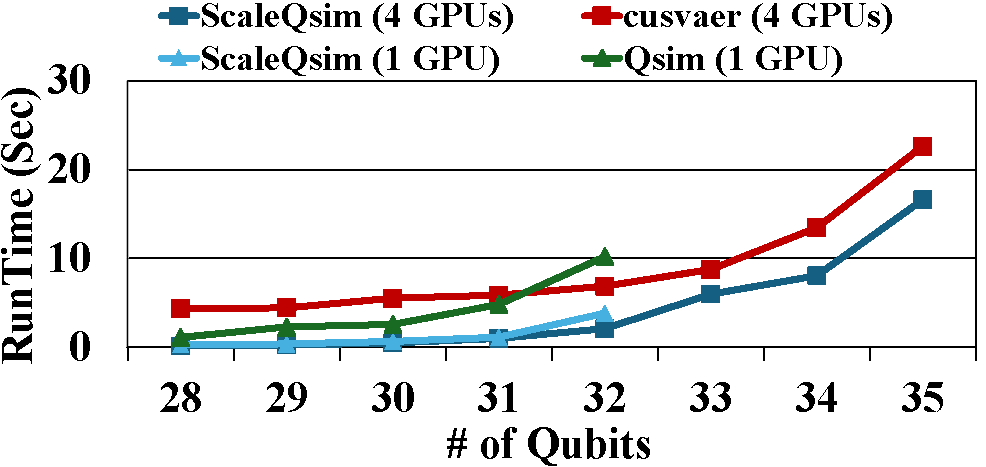
\includegraphics[width=13.3cm]{figures/MultiGPU_qsim.png}
  %\vspace{-.1cm}
  \captionsetup{skip=2pt}
  \caption{Scale-in: Multi-GPU support enables simulation of a higher number of qubits
  (log-scale).}
  \label{multigpu_perf}
  %\vspace{-.5cm}
\end{figure}

\noindent
\textbf{Comparison with \textit{HyQuas} and \textit{Atlas}.} At 30 qubits on 4
GPUs, \ScaleQsim achieves 1.32$\times$ and 1.73$\times$ speedup over \textit{HyQuas}
and \textit{Atlas}, respectively. However, as the number of qubits increases, both
SOTA simulators fail to scale: \textit{HyQuas} cannot simulate beyond 32 qubits on
1 GPU or 30 qubits on 4 GPUs, while \textit{Atlas} fails to execute above 30 qubits
in all configurations. In contrast, \ScaleQsim successfully completes simulation
up to 32 qubits on 1 GPU in 2.57 seconds and on 4 GPUs in 0.99 seconds, which
demonstrates both its successful execution at larger scales and its superior
scalability. The limitation of \textit{HyQuas} and \textit{Atlas} is caused not by
insufficient memory, but by the underlying design of each simulator. A100 GPU (80
GB) is equipped with sufficient memory for up to 33-qubit simulations (e.g.,
16–64 GB for 31–33 qubits in single precision, 8 bytes per complex amplitude). Thus,
the non-executable of \textit{\textit{HyQuas}} beyond 30 (4 GPUs), 32 qubits (1 GPU),
and \textit{Atlas} beyond 30 qubits (1, 4 GPUs) is not caused by memory limitations,
but by structural inflexibility in statically defined kernel structures and
fixed simulation plans.

%Specifically, \textit{\textit{HyQuas}} divides a large circuit into sub circuits and simulates them using precompiled kernels with a fixed number of local qubits and statically allocated memory layouts.
%However, as the number of total qubits increases, it creates a large sub-circuit that cannot fit into the total memory of a single GPU.
%When the size of the sub-circuit exceeds this fixed configuration, kernel execution fails due to internal overflow in offset tables or shared memory allocation.
%Specifically, \textit{HyQuas} fuses a set of gates into precompiled kernels, each designed to operate on a fixed number of local qubits with statically allocated memory layouts.
%However, as the number of total qubits increases, each GPU is assigned a larger portion of the state vector, which implicitly increases the number of local qubits it should manage (e.g., 2\textsuperscript{36} / 4 GPUs = 2\textsuperscript{34} amplitudes → 34 local qubits).
%When this exceeds the kernel’s preconfigured limit (e.g., 28 local qubits), execution fails due to internal overflow in offset tables or shared memory allocation.

Specifically, \textit{HyQuas} divides the circuit into sub-circuits, each
composed of a partitioned group of gates, and simulates them using precompiled kernels
with a fixed number of local qubits (e.g., 28) and statically allocated memory layouts.
However, as the number of total qubits increases, some sub-circuits require more
local qubits than the kernel can handle, and the corresponding sub-circuit exceeds
the available memory on a single GPU. When a sub-circuit accesses more qubits
than the kernel is designed to process, execution fails due to internal overflow
in offset tables or shared memory allocation.

Similarly, \textit{Atlas} adopts a strict gate-to-qubit mapping scheme and constructs
a fixed simulation plan based on a predefined GPU configuration. To overcome the
fixed plan limitation, we also attempted to generate a simulation plan on a single
A100 (80~GB) using the identical setup, but \textit{Atlas} failed to produce a valid
simulation plan and timed out. This is further supported by our evaluation
results that only the specific qubit-GPU combinations described in the paper~\cite{xu2024atlas}
executed successfully in our evaluation setup, while other combinations failed to
generate a simulation plan, even when using the identical computing setup. These
findings reveal the inflexibility of static simulation plans, which fail to
accommodate varying circuit sizes or hardware configurations. As the number of qubits
increases, the mismatch between the required state vector size and available GPU
memory, combined with the lack of dynamic scheduling, leads to memory conflicts
and simulation failure.

In contrast, \ScaleQsim supports dynamic and scalable execution by computing affected
\texttt{Target Indices} at runtime and adaptively configuring kernel parameters,
including CUDA thread-block structures. Based on the requested number of qubits,
\ScaleQsim dynamically calculates the required memory size and evenly distributes
the state vector, prior to the simulation execution. This dynamic state vector management
allows \ScaleQsim to evenly distribute gate execution without skewness.

\subsection{Multi-Node Scalability}
%\vspace{-.1cm}

\begin{figure*}[t]
  \centering
  % Legend 이미지 (첫 번째 행)
  \begin{subfigure}
    [b]{9.5cm}
    \centering
    \includegraphics[width=\textwidth]{figures/legend.png}
  \end{subfigure}
  %\vspace{-.3cm}

  % 서브플롯 4개
  \begin{subfigure}
    [b]{3.35cm}
    \centering
    \includegraphics[width=\textwidth]{figures/qft_weak.png}
    \caption{qft.}
    \label{qft_weak}
  \end{subfigure}
  \begin{subfigure}
    [b]{3.35cm}
    \centering
    \includegraphics[width=\textwidth]{figures/vqc_weak.png}
    \caption{vqc.}
    \label{vqc_weak}
  \end{subfigure}
  \begin{subfigure}
    [b]{3.35cm}
    \centering
    \includegraphics[width=\textwidth]{figures/qsvm_weak.png}
    \caption{qsvm.}
    \label{qsvm_weak}
  \end{subfigure}
  \begin{subfigure}
    [b]{3.35cm}
    \centering
    \includegraphics[width=\textwidth]{figures/ghz_weak.png}
    \caption{ghz.}
    \label{ghz_weak}
  \end{subfigure}
  %\vspace{-.3cm}

  \caption{Weak scalability of \ScaleQsim and SOTA across diverse circuits and
  GPU scales (log-scale).}
  \label{compared_cusvaer_2}
  %\vspace{-0.6cm}
\end{figure*}

\noindent
\textbf{Weak scalability with various circuits.} Figure~\ref{compared_cusvaer_2}
compares the weak scalability of \ScaleQsim with SOTA simulators (\textit{cusvaer},
\textit{HyQuas}, \textit{Atlas}) across four circuit types: qft, vqc, qsvm, and ghz.
qft and vqc are high-complexity circuits, characterized by strong inter-qubit interactions
and large gate counts, while qsvm and ghz represent lower-complexity circuits
with simpler execution flows. We varied both the number of qubits and GPUs simultaneously
(e.g., from 28 qubits on 1 GPU to 36 qubits on 256 GPUs) to evaluate how each simulator
maintains performance under increasing problem size and resource scale. The
comparison focuses on how the scalability trend varies depending on circuit
characteristics.

As shown in the figure, for high-complexity circuits, in qft, \ScaleQsim takes 0.26s
at 28 qubits and 1.41s at 36 qubits. At 36 qubits, \ScaleQsim achieves 15.63$\times$
and 6.62$\times$ speedup over \textit{cusvaer} (22.05s) and \textit{HyQuas} (9.34s),
respectively. However, \textit{Atlas} achieves the lowest simulation time of 1.10s
at 36 qubits, slightly outperforming \ScaleQsim in this specific case. In vqc, \ScaleQsim
maintains stable simulation time, from 0.16s (28 qubits) to 1.18s (36 qubits). At
36 qubits, it achieves 18.30$\times$, 11.00$\times$, and 2.40$\times$ speedup over
\textit{cusvaer} (21.67s), \textit{HyQuas} (12.95s), and \textit{Atlas} (2.88s),
respectively. For low-complexity circuits, in qsvm, \ScaleQsim takes 0.05s at 28
qubits and 0.99s at 36 qubits, achieving up to 19.00$\times$, 9.70$\times$, and
1.30$\times$ speedup over \textit{cusvaer} (18.83s), \textit{HyQuas} (9.63s), and
\textit{Atlas} (1.26s), respectively. In ghz, \ScaleQsim completes the 36-qubit
simulation in 1.08s, achieving 16.60$\times$ and 10.20$\times$ speedup over
\textit{cusvaer} (17.94s) and \textit{HyQuas} (11.04s), while \textit{Atlas}
achieves the lowest simulation time (0.82s) in this specific case. \textit{Atlas}
achieves the best performance in specific configurations that utilize a precompiled
simulation plan. However, since \textit{Atlas} has to first produce the plan
before the execution in a realistic scenario, its total runtime would increase due
to the newly included plan generation time.
%This is because it failed to produce a valid simulation plan, even using an identical evaluation setup.
%Since \textit{Atlas} has to first produce the plan before the execution in a realistic scenario, its total runtime would increase due to the newly included plan generation time.

These results show how circuit characteristics influence simulator scalability.
Specifically, in qft, strong inter-qubit interactions arise due to controlled-phase
gates, where each qubit interacts with all lower qubits~\cite{rached2025characterizing,
jin2023quantum}. This structure favors \textit{Atlas}, which statically defines
execution paths within local qubit partitions to minimize communication overhead.
Although \textit{Atlas} was slightly faster, the performance gap with \ScaleQsim
remained small (1.10s vs. 1.41s at 36 qubits), demonstrating that static and even
distribution of memory layout across GPUs does not incur too much overhead due to
replicated mapping between local and global and efficient protocol usage. In
contrast, vqc contains many gate operations but exhibits low inter-qubit interactions,
as most gates are single-qubit or local entangling gates confined to adjacent
qubits~\cite{kandala2017hardware, zuniga2024variational}. This structure favors \ScaleQsim,
which executes operations independently based on affected \texttt{Target Indices},
enabling many gate operations to process within each GPU and reducing
synchronization and cross-node communication. In addition, qsvm and ghz are
relatively lower-complexity as simple entanglement structures. qsvm include many
gates, but most are local operations with weak inter-qubit interactions, while ghz
contain shallow entanglement that spans all qubits, but a low number of gates. These
characteristics allow \ScaleQsim to maintain scalability by minimizing cross-node
communication and ensuring efficient task execution across GPUs. However, \textit{cusvaer}
and \textit{HyQuas} show consistent performance degradation regardless of circuit
characteristics. \textit{cusvaer} suffers from overhead caused by memory pooling
and centralized gate scheduling, while \textit{HyQuas} causes overhead from global-local
swap operations that trigger frequent cross-node shuffling as the number of nodes
increases.

\begin{figure*}[t]
  \centering
  % Legend 이미지 (첫 번째 행)
  \begin{subfigure}
    [b]{9.5cm}
    \centering
    \includegraphics[width=\textwidth]{figures/legend.png}
  \end{subfigure}
  %\vspace{-0.3cm}

  % 서브플롯 4개
  \begin{subfigure}
    [b]{3.35cm}
    \centering
    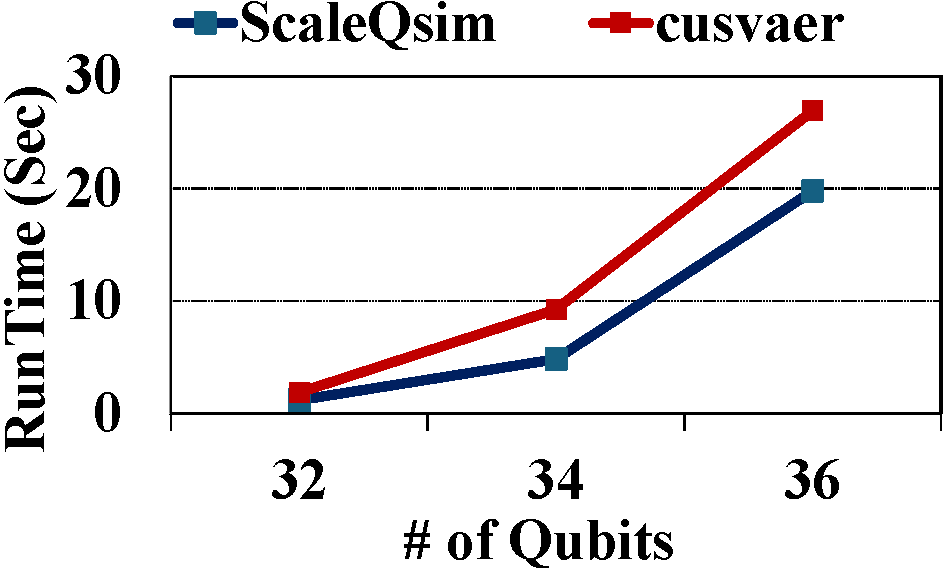
\includegraphics[width=\textwidth]{figures/16gpus.png}
    \caption{16 GPUs.}
    \label{16gpus}
  \end{subfigure}
  \begin{subfigure}
    [b]{3.35cm}
    \centering
    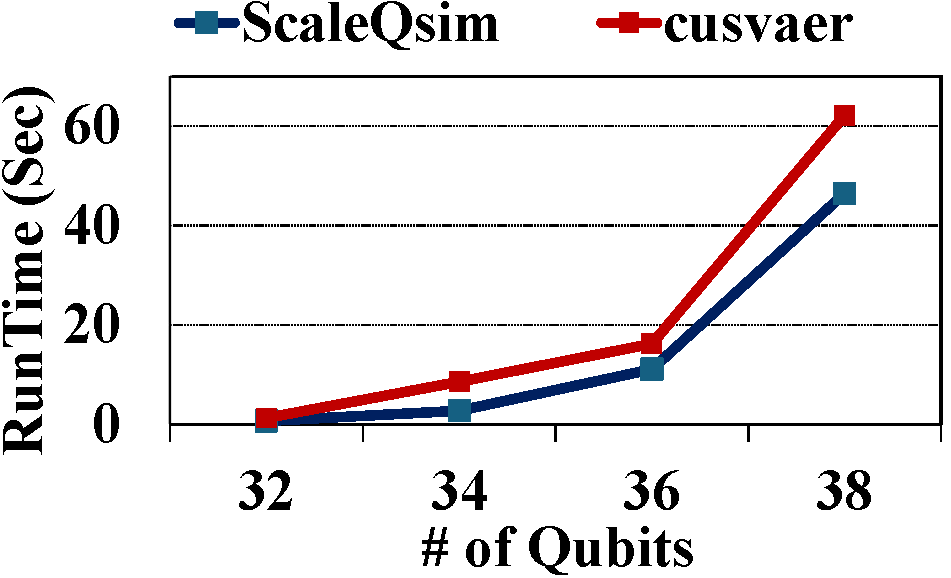
\includegraphics[width=\textwidth]{figures/32gpus.png}
    \caption{32 GPUs.}
    \label{32gpus}
  \end{subfigure}
  \begin{subfigure}
    [b]{3.35cm}
    \centering
    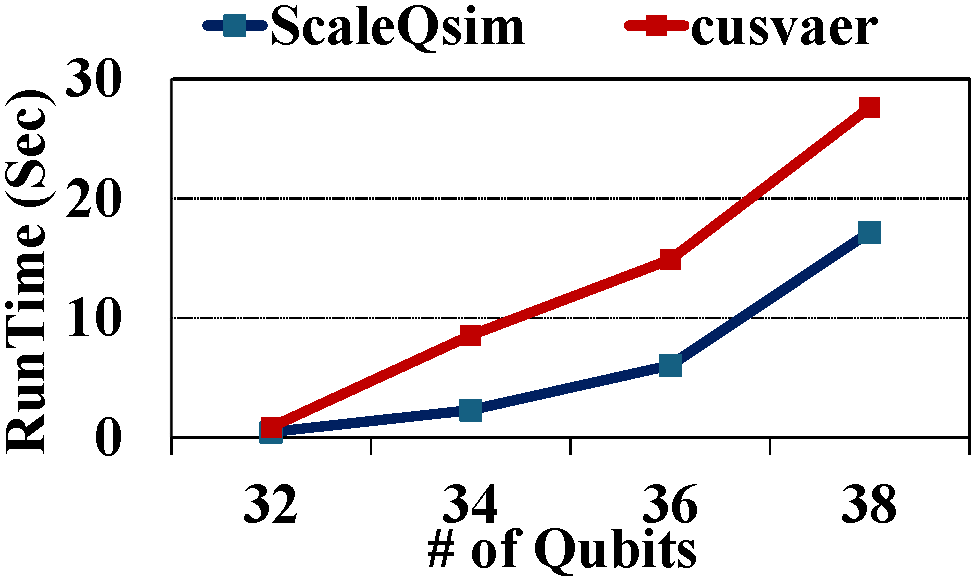
\includegraphics[width=\textwidth]{figures/64gpus.png}
    \caption{64 GPUs.}
    \label{64gpus}
  \end{subfigure}
  \begin{subfigure}
    [b]{3.35cm}
    \centering
    \includegraphics[width=\textwidth]{figures/256gpus.png}
    \caption{256 GPUs.}
    \label{128gpus}
  \end{subfigure}
  %\vspace{-.3cm}
  \caption{Strong scalability comparison of \ScaleQsim and SOTA on qft circuits
  with the number of GPUs.}
  \label{compared_cusvaer_1}

  %\vspace{-0.6cm}
\end{figure*}

\noindent
\textbf{Strong scalability with multiple GPUs.} Figure~\ref{compared_cusvaer_1} compares
the strong scalability of \ScaleQsim, \textit{cusvaer}, \textit{HyQuas}, and
\textit{\textit{Atlas}} with an increasing number of qubits across varying numbers
of GPUs from 16 to 256 GPUs. As shown in the figure, \ScaleQsim consistently outperforms
\textit{cusvaer} across all configurations. \changjong{At 16 GPUs, \ScaleQsim takes 18.58 seconds at 36 qubits, compared to 36.62 seconds by \textit{cusvaer}, showing a 1.97$\times$ speedup.}
At 32 and 64 GPUs, the simulation time at 38 qubits is 37.43 and 14.16 seconds for
\ScaleQsim, and 62.14 and 27.61 seconds for \textit{cusvaer}, resulting in 1.70$\times$
and 1.95$\times$ speedups, respectively. With 256 GPUs, \ScaleQsim completes the
40-qubit simulation in 33.01 seconds, while \textit{cusvaer} takes 68.46 seconds,
achieving a 2.10$\times$ speedup. These results demonstrate that \ScaleQsim
provides lower simulation time and better scalability across a wide range of
configurations, particularly as the number of qubits increases.

In contrast, \textit{\textit{HyQuas}} and \textit{\textit{Atlas}} exhibit severe
limitations in strong scalability due to their static kernel configurations and
memory layouts. \textit{HyQuas} fails to execute beyond 36-qubit simulation in
most configurations and only completes a 36-qubit simulation on 256 GPUs with a
simulation time of 9.34 seconds. In contrast, \ScaleQsim performs the same
simulation in 1.41 seconds, achieving a 6.6$\times$ speedup. Notably, all 38- and
40-qubit simulations fail on \textit{HyQuas}, regardless of the number of GPUs.
These failures stem from its use of precompiled CUDA kernels with fixed local
qubit (e.g., 28 qubits), which are statically embedded in both kernel design and
scheduling logic, restricting scalability to larger or irregular circuits. \textit{Atlas}
also demonstrates limited scalability. Executable configurations are limited to 32-qubit
on 16 GPUs (0.63s), 34-qubit on 64 GPUs (0.89s), and 36-qubit on 256 GPUs (1.09s).
%All other configurations of qubits and GPUs fail to execute due to strict gate-to-qubit mapping and static scheduling constraints.
All other configurations of qubits and GPUs fail to execute due to the architectural
constraints discussed in Section~\ref{singlenodeperf}.

\begin{comment}
\skim{ \textbf{Replace this whole part by just saying "due to  to above mentioned reasons?}
This limitation does not result from insufficient GPU memory. The available memory on A100 with 80 GB per device is sufficient to support 36-qubit simulations (512 GB) on 16 GPUs (1.2 TB total) and 40-qubit simulations (8 TB) on 128 GPUs (10.24 TB total). The root cause lies in architectural inflexibility, including static kernel configurations and fixed memory layouts, fixed gate-to-qubit mappings, and a lack of simulation time adaptability, all of which limit resource utilization.
}    
\end{comment}

Despite its current inability to execute, we believe the divide and conquer approach
of \textit{Atlas} will face scalability issues similar to those of \textit{HyQuas},
even if executed correctly at a higher number of qubits. As the circuit size grows,
we anticipate it will become difficult to generate efficient sub-circuits, leading
to three problems. 1) The divided sub-circuits will become imbalanced, causing
workload skewness. 2) As the number of sub-circuits grows, distributed execution
will increase communication and synchronization overhead. 3) Individual sub-circuits
will be too large to fit into a GPU memory. This will cause simulation failures
at a lower qubit count compared to \ScaleQsim, even when using an identical number
of GPUs. Thus, these results highlight that \ScaleQsim is the only simulator in the
evaluation that supports scalable and high-performance execution up to 40-qubit simulation
with 256 GPUs, while maintaining performance advantages over all baselines.

%We also attempted to generate a simulation plan with up to 33 local qubits on a single A100 (80 GB) using the identical computing setup, but \textit{Atlas} failed to produce a valid simulation plan.
%This is further supported by our finding that only the specific qubit-GPU combinations described in the paper~\cite{xu2024atlas} executed successfully in our evaluation setup, while other combinations failed to generate a simulation plan, even when using the identical computing setup.

\subsection{Performance and Scalability in Diverse Circuit Comparison with SOTA
(\textit{cusvaer})}
%\vspace{-.1cm}

%\skim{Change 4.4 and 4.5 into Comparison with SOTA and use subsubsection of Scalablity and Different Circuits?}

%\skim{DATA presention in this section is dirty, can we just present that last data only? largest qubit for every sceanrio (GPU and circutis). and give only times}
\begin{comment}
 \noindent\textbf{Scalability: }Figure~\ref{compared_cusvaer_1} compares the simulation time scalability of \ScaleQsim and \textit{cusvaer} with an increasing number of qubits across varying numbers of GPUs from 16 to 128 GPUs. As shown in the figure, \ScaleQsim consistently outperforms \textit{cusvaer} across all configurations.
At 16 GPUs, \ScaleQsim takes 19.78 seconds at 36 qubits, compared to 26.91 seconds by \textit{cusvaer}, showing a 1.36$\times$ speedup.
At 32 and 64 GPUs, the simulation time at 38 qubits is 46.44 and 14.16 seconds for \ScaleQsim, and 62.14 and 27.61 seconds for \textit{cusvaer}, resulting in 1.34$\times$ and 1.95$\times$ speedups, respectively.
With 128 GPUs, \ScaleQsim completes the 40-qubit simulation in 39.66 seconds, while \textit{cusvaer} takes 56.28 seconds, achieving a 1.42$\times$ speedup.
These results demonstrate that \ScaleQsim provides lower simulation time and better scalability across a wide range of configurations, particularly as the number of qubits increases.
   
\end{comment}

\begin{comment}
In addition, \ScaleQsim consistently outperforms \textit{cusvaer} when using 64 and 128 GPUs. For 64 GPUs, \ScaleQsim achieves simulation times of 14.16 seconds and 85.65 seconds for 38 and 40 qubits, while \textit{cusvaer} records 27.60 seconds and 159.47 seconds, yielding speedups of 1.95$\times$ and 1.86$\times$, respectively. For 128 GPUs, \ScaleQsim completes the 40-qubit simulation in 39.66 seconds, compared to 56.28 seconds by \textit{cusvaer}, achieving a speedup of 1.42$\times$. This is because \ScaleQsim evenly partitions the state vector across all GPUs, ensuring balanced memory usage and reducing overload on specific devices as the state vector grows exponentially. In contrast, \textit{cusvaer} uses a memory pooling strategy, where the state management information is handled by a single node and creates uneven memory allocation across distributed GPUs. This can lead to memory fragmentation or misalignment,  even when total memory capacity seems sufficient.  
\end{comment}

\begin{comment}
  \begin{figure*}[t]
    \centering
    \subfloat[qft.]{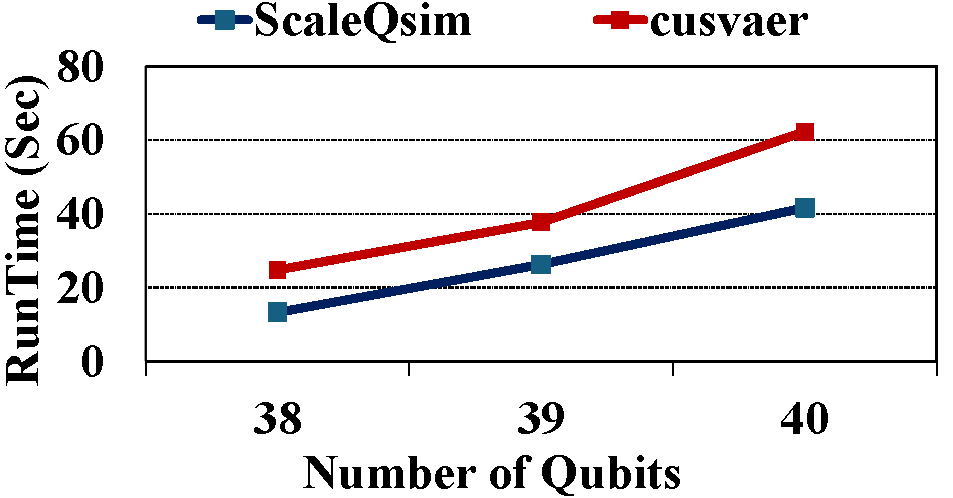
\includegraphics[width=5.5cm]{figures/qft.pdf}\label{qft}}%
    \subfloat[qv.]{\includegraphics[width=5.5cm]{figures/qv.pdf}\label{qv}}%
    \subfloat[vqc.]{\includegraphics[width=5.5cm]{figures/vqc.pdf}\label{vqc}}%
    \\ % 줄바꿈
    \subfloat[qsvm.]{\includegraphics[width=5.5cm]{figures/qsvm.pdf}\label{qsvm}}%
    \subfloat[random.]{\includegraphics[width=5.5cm]{figures/random.pdf}\label{random}}%
    \subfloat[ghz.]{\includegraphics[width=5.5cm]{figures/ghz.pdf}\label{ghz}}%
  \caption{Performance Compared to cusvaer using 128GPU} %\skim{maybe break this two different figures?}
  \label{compared_cusvaer_various}
\end{figure*}      
\end{comment}

\begin{comment}
\begin{figure*}[t]
    \centering
    \subfloat[16 GPU.]{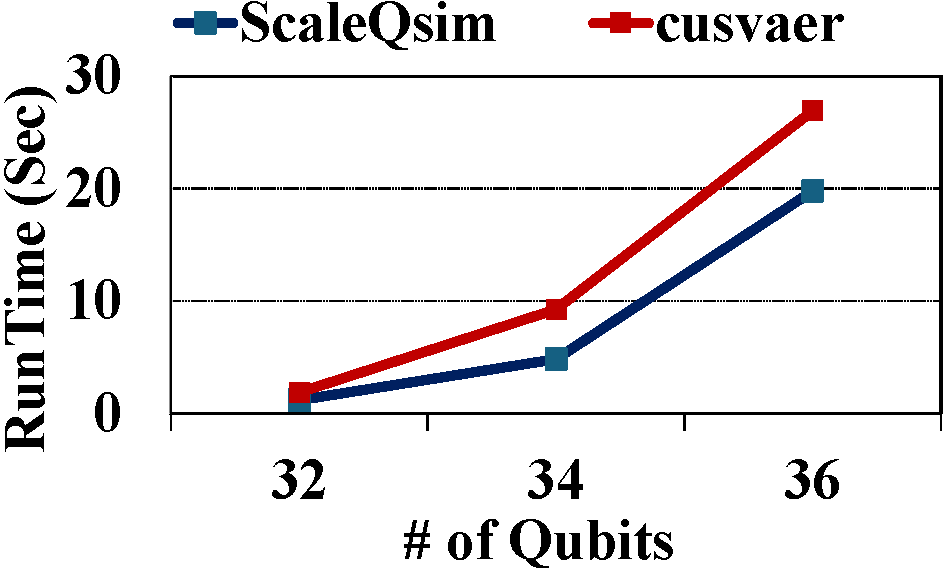
\includegraphics[width=3.85cm]{figures/16gpus.pdf}\label{16gpus}}%
    \centering
    \subfloat[32 GPU.]{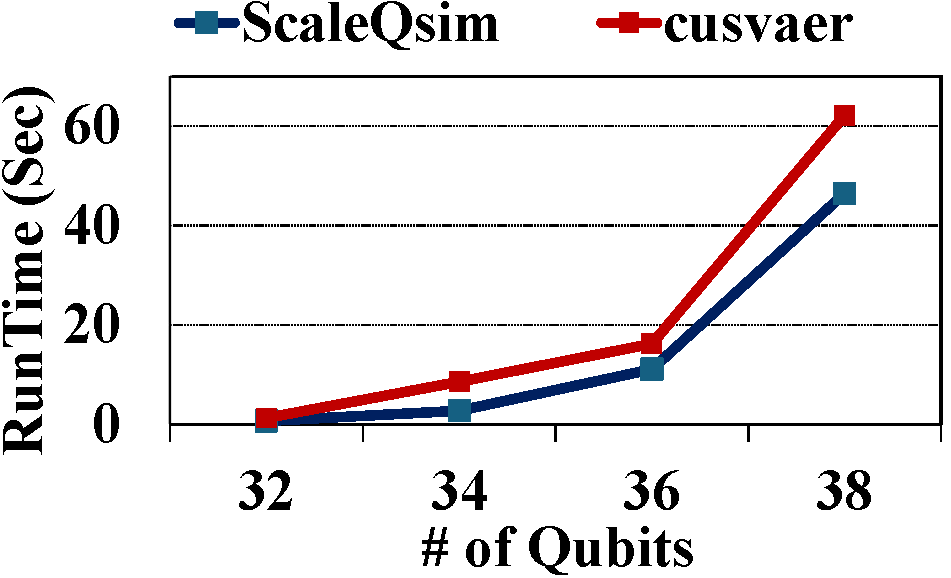
\includegraphics[width=3.80cm]{figures/32gpus.pdf}\label{32gpus}}%
    \centering
    \subfloat[64 GPU.]{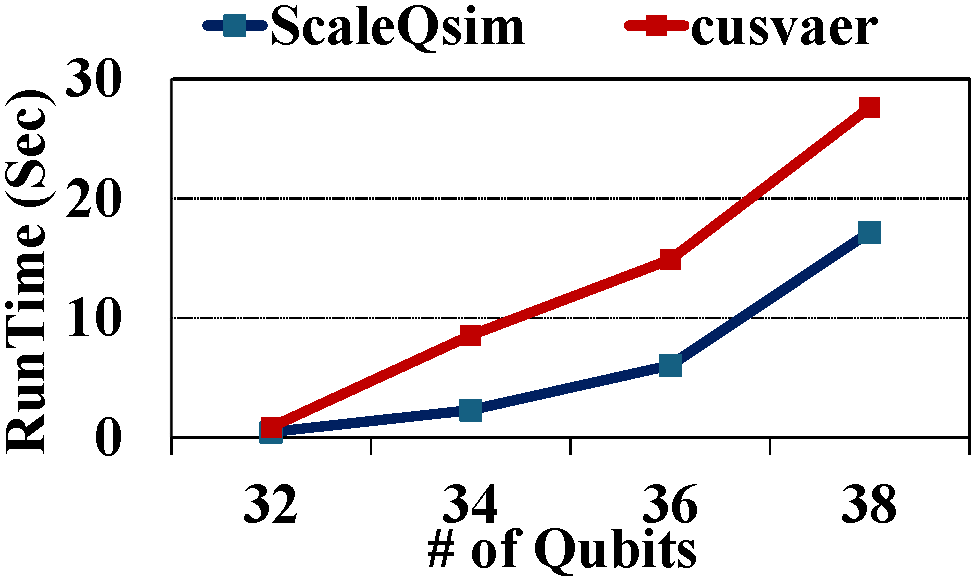
\includegraphics[width=3.90cm]{figures/64gpus.pdf}\label{64gpus}}%
    \centering
    \subfloat[128 GPU.]{\includegraphics[width=3.90cm]{figures/128gpus.pdf}\label{128gpus}}%

  \caption{Performance comparison between \ScaleQsim and \textit{cusvaer} for qft circuits across multiple GPU setups.} 
     
  \label{compared_cusvaer_1}

\end{figure*}     
\end{comment}

\changjong{ Figure~\ref{compared_cusvaer_various} compares the simulation performance of \ScaleQsim and \textit{cusvaer} across six representative quantum circuits: qv, vqc, qsvm, random, ghz, and vqe.}
Note that \textit{HyQuas} and \textit{Atlas} are excluded from this comparison, as
both simulators fail to execute circuits with 38 qubits or more in most configurations
due to their architectural constraints. All experiments were conducted on the
identical 128 GPUs (32 nodes). As shown in the figure, for the 38–40 qubit range,
\ScaleQsim consistently outperformed \textit{cusvaer} across all circuits. At 40
qubits, \ScaleQsim and \textit{cusvaer} take 29.92 and 65.39 seconds for qv circuit,
achieving a 2.19$\times$ speedup. For vqc and qsvm, they take 21.55 and 22.37 seconds,
while \textit{cusvaer} takes 34.97 and 37.69 seconds, resulting in 1.62$\times$ and
1.69$\times$ speedups, respectively. Random circuit takes 5.66 and 19.02 seconds,
yielding a 3.36$\times$ speedup, and ghz circuit takes 12.52 and 23.24 seconds,
achieving a 1.86$\times$ speedup. \changjong{For vqe, \ScaleQsim takes 80.57 seconds, while \textit{cusvaer} takes 98.29 seconds, resulting in a 1.21$\times$ speedup.}
Although performance varies across circuit types, \ScaleQsim demonstrated
consistent performance improvements up to 6.15$\times$ over \textit{cusvaer}.

\begin{figure*}[t]
  \centering
  % 첫 줄: 3개
  \subfloat[qv.]{\includegraphics[width=4.35cm]{figures/qv.png}\label{qv}}
  \hspace{0.3cm} \subfloat[vqc.]{\includegraphics[width=4.35cm]{figures/vqc.png}\label{vqc}}
  \hspace{0.3cm} \subfloat[qsvm.]{\includegraphics[width=4.35cm]{figures/qsvm.png}\label{qsvm}}

  % 두 번째 줄: 2개
  \subfloat[random.]{\includegraphics[width=4.35cm]{figures/random.png}\label{random}}
  \hspace{0.3cm} \subfloat[ghz.]{\includegraphics[width=4.35cm]{figures/ghz.png}\label{ghz}}
  \subfloat[\changjong{vqe.}]{\includegraphics[width=4.35cm]{figures/vqe.png}\label{vqe}}
  %\vspace{-.3cm}

  \caption{Performance comparison between \ScaleQsim and \textit{cusvaer} across
  diverse circuits using 128 GPUs.}
  \label{compared_cusvaer_various}
  %\vspace{-.5cm}
\end{figure*}

\changjong{ Notably, \ScaleQsim showed significant performance improvements over \textit{cusvaer} for ghz and random. This is because ghz has low depth and a simple linear structure based on CNOT gates, resulting in low computational complexity and minimal memory access. In random circuits, although gate-to-qubit mappings are randomized, many operations remain localized to a small subset of qubits, reducing the need for inter-communication. This locality aligns well with \texttt{Target Index}-based execution scheme, enabling efficient parallelization with minimal data movement. In contrast, qv, vqc, qsvm, and vqe have deeper structures and broader qubit interactions, often involving multiple controlled gates. These characteristics increase both computational load and inter-communication. However, \ScaleQsim maintains consistent performance by precomputing \texttt{Target Indices} to access only necessary amplitudes and applying adaptive kernel tuning to maximize thread-level parallelism in regions with heavier workloads.

Additionally, \ScaleQsim shows reduced speedup on vqe circuits compared to less gate-intensive circuits. This is because, although the circuit primarily consists of communication-efficient local gates (e.g., single-qubit or adjacent entangling operations), its performance is limited by the heavy computational load from its thousands of gate operations. Despite this, \ScaleQsim still outperforms \textit{cusvaer} on vqe circuit. \ScaleQsim effectively exploits circuit locality through its \texttt{Target Index}-based execution, enabling local operations to run independently within each GPU partition and reducing coordination and cross-node communication. In contrast, \textit{cusvaer} incurs overhead from memory pooling and centralized gate scheduling, which limits its ability to leverage communication-efficient circuits and causes lower performance. }
%As a result, \ScaleQsim shows high scalability and consistent performance across both simple and complex quantum circuits, showing its ability to adapt effectively to a wide range of quantum algorithms.
\begin{comment}
 Notably, \ScaleQsim showed significant performance improvements over \textit{cusvaer} for the ghz and random circuits. This is because ghz circuit consists of a low circuit depth and a simple linear structure based on CNOT gates, leading to low computational complexity and minimal memory access. 
For a random circuit, although gate-to-qubit mappings are randomized, many operations remain localized to a small set of qubits, reducing the need for inter-communication. This locality matches well with the target index-based execution scheme, allowing efficient parallelization with minimal data movement. In contrast, qv, vqc, and qsvm circuits have deeper structures and wider qubit interactions, often involving many controlled gates. 
These characteristics increase both the overall computation and the amount of inter-communication required. 
However, \ScaleQsim still achieves consistent performance by precomputing \texttt{Target Indices} to process only the necessary amplitudes and by applying adaptive kernel tuning. This approach maximizes thread-level parallelism, especially in regions with heavier workloads, and reduces unnecessary memory and communication overhead.   
\end{comment}

\subsection{Extreme Scale-out: Multiple-Nodes}
%\vspace{-.1cm}

\begin{comment}

With 8 GPUs, \ScaleQsim completes simulations for up to 38 qubits, taking 84.8 seconds. Simulations for more than 38 qubits cannot be executed due to memory limitations.
For 16 GPU and 32 GPU, \ScaleQsim scales to 39 and 40 qubits, completing in 178.8 and 159.5 seconds, respectively. Notably, 32GPU achieves lower simulation time than 16GPU at 39 qubits (95.9, 178.8 seconds), demonstrating more efficient scaling.
For 64 GPU and 128 GPU, simulations scale up to the full 42 qubits, completing in 251.1 and 160.5 seconds, respectively.

As the number of GPUs increases, \ScaleQsim successfully overcomes the 32-qubit limit typical of single-node simulators, extending the maximum simulatable number of qubits up to 42 by leveraging scale-out across multiple nodes. Specifically, \ScaleQsim expands the simulation capacity from 38 qubits with 8 GPU to the full 42 qubits with 128 GPU.
However, for 64 GPU and 128 GPU, performance degradation is observed beyond 40 qubits, primarily due to the exponential increase in computational task size, with some additional impact from communication overhead. 
Despite, At 40, 41, and 42 qubits, the 128 GPU achieves speedups of 1.63$\times$, 1.76$\times$, and 1.56$\times$ over the 64 GPU, respectively. 
\skim{We also have to mention why performance of odd number qubit is bad.}
These results show that \ScaleQsim effectively utilizes scale-out to handle increasing computational demands, enabling performance gains and scalable simulation of a higher number of qubits.

    
\end{comment}

Figure~\ref{multinode_perf} shows the simulation time performance of \ScaleQsim as
the number of qubits increases from 32 to 42 using qft circuits, evaluated
across 8 to 512 GPUs. \ScaleQsim scales from 2 nodes (8 GPUs) up to 32 nodes (128
GPUs) for up to 40 qubits and further extends to 256 and 512 GPUs for 41 and 42 qubits,
respectively, demonstrating its ability to support large-scale simulations beyond
40 qubits. As shown in Figure~\ref{multinode_a}, \ScaleQsim scales efficiently as
the number of GPUs increases, both in terms of the number of supported qubits
and simulation time. It supports up to 36 qubits with 8 GPUs and up to 40 qubits
with 128 GPUs. This scale-out execution overcomes single-node memory limitations
and enables full state simulations at larger scales. In terms of simulation time
scalability, \ScaleQsim achieves lower simulation times as the number of GPUs
increases.

%\skim{\textbf{Original}
%For example, at 36 qubits, the simulation time decreases from 32.42 seconds on 8 GPUs to 4.28 seconds on 128 GPUs.
%\skim{\textbf{Original}
%At 39 qubits, the simulation time is reduced from 52.54 seconds on 64 GPUs to 29.22 seconds on 128 GPUs.
%This corresponds to speedups of 7.57$\times$ at 36 qubits and 1.80$\times$ at 39 qubits.
%}
%}
%\skim{\textbf{New}

\begin{figure}[t]
  \centering
  \subfloat[32--40 Qubits.]{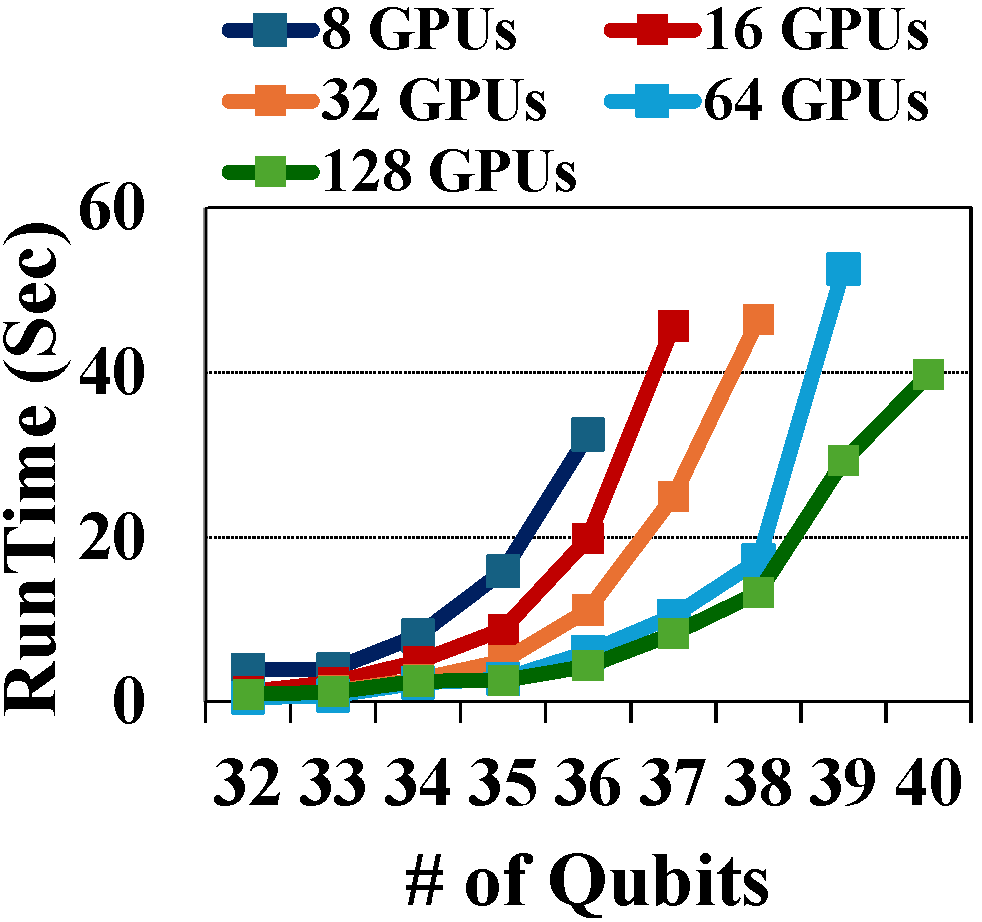
\includegraphics[width=9.5cm]{figures/multinode_perf.png}\label{multinode_a}}%
  \subfloat[41--42 Qubits.]{\includegraphics[width=3.05cm]{figures/multinode_perf_b.png}\label{multinode_b}}%
  %\vspace{-.3cm}

  \caption{Scale-out: Multi-node support enables simulation of a higher number of
  qubits.}

  \label{multinode_perf}
  %\vspace{-.5cm}
\end{figure}

For the 36-qubit simulation, a 16-fold increase in GPUs (from 8 to 128) reduces the
simulation time from 32.42 to 4.28 seconds, achieving a 7.57$\times$ speedup.
The scalability is less than the linear ideal due to the initial GPU memory
allocation and coordination overhead becoming a bottleneck. However, the
scalability increases as the number of qubits increases. At 39 qubits,
\ScaleQsim achieves a 1.80$\times$ speedup, reducing simulation time from 52.54s
(64 GPUs) to 29.22s (128 GPUs). This shows that \ScaleQsim can effectively utilize
an increased number of GPUs to reduce simulation time.

Additionally, as shown in Figure~\ref{multinode_b}, \ScaleQsim achieves scalability
beyond 40 qubits by leveraging additional GPUs. When doubling the resources from
256 to 512 GPUs and the problem size from a 41 qubit (16 TB) to a 42 qubit (32 TB),
the simulation time for \ScaleQsim increased by only 28\% (from 81.25s to 104.31s).
This efficiency is due to two key designs. First, a \textit{Two-phase
Partitioning} strategy evenly distributes the full state vector across all GPUs
and maintains a constant 64 GB workload per GPU for both evaluations. Second, by
precomputing and broadcasting all necessary metadata using \textit{Statespace
Structure}, \ScaleQsim eliminates the need for computation path exploration or
global synchronization. However, the increase in simulation time is caused by
unavoidable communication overheads, such as MPI broadcast latency that grows with
the number of nodes and inter-node communication from larger gates that span multiple
nodes.

\begin{comment}
\changjong{
\ScaleQsim simulates a 41-qubit (16 TB) on 256 GPUs, in 81.25.
By doubling the resources to 512 GPUs, it can simulate a 42-qubit (a problem twice as large at 32 TB), with the simulation time increasing by only 28\% to 104.31 seconds. 
This relatively small gap in simulation time increase, despite a doubling in problem size, demonstrates the efficiency of \ScaleQsim in large-scale simulations. 
Two key factors contribute to this scalability:
(1)~\textit{Two-phase Partitioning} strategy evenly distributes the exponentially growing state vector across all GPUs. For both 41-qubit (16TB, 256 GPUs) and 42-qubit (32TB, 512 GPUs) simulations, each GPU handles the identical 64 GB space, ensuring a consistent per-GPU workload and reducing simulation time increases.
(2)~\textit{Statespace Structure} precomputes all \texttt{Target Indices} and broadcasts metadata to all nodes, removing the need for computation path exploration or global synchronization. However, some increase in simulation time is inevitable due to additional overhead introduced by the expanded scale. This is because, as the number of nodes doubles, MPI broadcast latency grows, and inter-node communication becomes more frequent for gates spanning multiple nodes. 
    
\end{comment}

%Despite \ScaleQsim minimizes the impact of these factors through precomputed task-to-GPU mappings and exclusive amplitude assignment, allowing it to maintain near-linear scalability across an increasing number of qubits.
%This highlights the efficiency of \ScaleQsim in handling large-scale simulations through balanced workload distribution and effective scaling.

%Although the state vector size doubles from 41 to 42 qubits, the simulation time increases by only 1.28$\times$, highlighting the efficiency of \ScaleQsim in handling large-scale simulations through balanced workload distribution and effective scaling.

%\skim{
%\ScaleQsim simulates a 41-qubit circuit (16 TB) on 256 GPUs in 81.25 seconds.
%By doubling the resources to 512 GPUs, it can simulate a 42 qubit circuit (a problem twice as large at 32 TB), with the time increasing by only 28\% to 104.31 seconds.
%}

\begin{comment}
\ScaleQsim demonstrates scalability in terms of the maximum number of qubits supported. With 8 GPUs, it completes simulations up to 38 qubits within available memory. 16 and 32 GPUs support 39 and 40 qubits, respectively. With 64 and 128 GPUs, \ScaleQsim successfully scales up to 42 qubits with 512 GPUs, overcoming the memory limitations of single-node simulators and enabling full-state simulations through scale-out execution.


In terms of simulation time scalability, \ScaleQsim achieves lower execution times as the number of GPUs increases. For example, at 39 qubits, the simulation time decreases from 178.8 seconds on 16 GPUs to 95.9 seconds on 32 GPUs. At 42 qubits, the simulation time is reduced from 251.1 seconds on 64 GPUs to 160.5 seconds on 128 GPUs. This corresponds to speedups of 1.63$\times$, 1.76$\times$, and 1.56$\times$ at 40, 41, and 42 qubits, respectively, compared to 64 GPUs.
These results show that \ScaleQsim effectively utilizes scale-out to handle increasing computational demands, enabling performance gains and scalable simulation of a higher number of qubits.    
\end{comment}

\subsection{Time Analysis}
%\vspace{-.1cm}
Since \ScaleQsim does not partition the circuit for independent local execution
within a single GPU, communication between nodes and GPUs can be frequent. Thus,
it is critical to minimize the communication overhead from the globally distributed
full state vector. To analyze the execution time of each subcomponent in
\ScaleQsim, Figure~\ref{time_analysis} presents the simulation time breakdown for
simulating a 38-qubit qft circuit across 32, 64, and 128 GPUs.~\changjong{We present the time breakdown by grouping the major components of the simulation into three distinct categories: Initialization (\textit{State Partitioning}, \textit{cudaMalloc}), Execution Planning (\textit{Task Aggregation}, \textit{Calculate Target Indices}), and Computation (\textit{Kernel Execution}, \textit{Intra-Communication}, \textit{Inter-Communication}). }

\begin{figure}[t]
  \centering
  \includegraphics[width=0.7\linewidth]{figures/time_result.png}
  \caption{\changjong{Time analysis using 38 qubits.}}
  \label{time_analysis}
  %\vspace{-0.35cm}
\end{figure}

\changjong{

\noindent\textbf{Initialization. }\textit{State Partitioning} time decreases as the number of GPUs increases, taking 0.34 seconds with 32 GPUs, 0.21 seconds (38.2\%) with 64 GPUs, and 0.17 seconds (50.0\%) with 128 GPUs. This reduction occurs because the task is parallelized, and a larger number of GPUs reduces the portion of the state vector handled by each GPU. In contrast, \textit{cudaMalloc} time increases from 0.76 seconds with 32 GPUs to 1.38 seconds (81.6\%) with 64 GPUs and 1.79 seconds (135.5\%) with 128 GPUs due to the additional overhead of managing memory allocation across more GPUs. Both component times account for only a small portion of the total simulation time. Additionally, this initialization process differs from \textit{Atlas}~\cite{xu2024atlas}, which relies on an offline process to generate a fixed simulation plan before execution. As the number of qubits and circuit complexity increase, this offline process grows significantly in duration, eventually taking longer than the execution time itself. In contrast, \ScaleQsim employs a lightweight initialization phase that simply partitions the full state vector based on the number of qubits and available GPUs, avoiding any time-consuming offline process before proceeding directly to the execution phase.

\noindent\textbf{Execution Planning. }\textit{Task Aggregation} time increases as the number of GPUs increases, taking 0.24, 0.48, and 0.88 seconds with 32, 64, and 128 GPUs, respectively. Similarly, \textit{Calculate Target Indices} time increases from 0.43 to 0.61 and 0.94 seconds with 32, 64, and 128 GPUs, respectively. This reflects the increased cost of calculating each \texttt{Target Index} to its physical location (i.e., a specific node and GPU) as the state vector is partitioned across more GPUs. However, the increases in planning time are not a significant bottleneck due to lightweight bitmask operations with minimal overhead, and the combined overhead from both components remains a small fraction of the total simulation time.

}

\noindent
\textbf{Computation. }\textit{Kernel Execution} occupies the largest portion of
the total simulation time. With 32 GPUs, it takes 39.13 seconds out of 44.67
seconds, accounting for approximately 87.58\% of the total time. As the number of
GPUs increases, \textit{Kernel Execution} time decreases to 10.77 seconds (60.06\%)
with 64 GPUs and 6.43 seconds (41.39\%) with 128 GPUs. This shows that
\ScaleQsim achieves high parallelism by distributing tasks across multiple nodes
and GPUs, which enables faster execution through efficient task partitioning and
concurrent processing. In contrast, communication overhead gradually increases as
the number of nodes and GPUs increases. \textit{Inter-Communication} measures the
execution time for three combined operations: broadcasting the metadata (\textit{Statespace
Structure}), performing a subsequent MPI coordination, and accessing remote memory
during gate operations that span multiple nodes. As the time required for all
three operations increases with the number of nodes, the total \textit{Inter-communication}
increases from 2.59 seconds (5.79\%) with 32 GPUs to 2.84 seconds (15.83\%) with
64 GPUs and 3.25 seconds (20.92\%) with 128 GPUs, as more nodes require data
transfer and MPI coordination. On the other hand, \textit{Intra-Communication} measures
communication between GPUs within the same node, a process that utilizes CUDA
peer-to-peer (P2P). As the number of qubits increases by utilizing more GPUs,
the size of the vector that represents each possible qubit state increases. Thus,
the state vector is distributed across multiple devices within a node, leading to
more frequent CUDA P2P access. This results in an increase in \textit{Intra-Communication}
time from 1.32 seconds (2.95\%) with 32 GPUs to 1.94 seconds (10.80\%) with 64 GPUs
and 2.26 seconds (14.55\%) with 128 GPUs.

\begin{comment}




Finally, the execution time spent on \textit{Calculate Target Indices} remains consistently low, recorded as 0.43, 0.61, and 0.94 seconds for 32, 64, and 128 GPUs, respectively, due to lightweight bitmask operations with minimal overhead. Similarly, the execution time for \textit{cudaMalloc + Initialization} increases slightly with more GPUs from 0.56, 0.82, and 1.08 seconds for 32, 64, and  128 GPUs, but accounts for only a small portion of the total simulation time.

 \begin{figure}[t]
    \centering
    \includegraphics[width=11.3cm]{figures/time_result.png}
    \caption{Time analysis using 38 Qubits.} %\skim{change the ordering. 16 gpu should come first}
    \label{time_analysis}
\end{figure}   

        
\begin{figure}[t]
    \centering
    \includegraphics[width=12.5cm]{figures/hitmap_ScaleQsim.png}
    \caption{Performance variability of \ScaleQsim and \textit{cusvaer}.}
    \label{consistency_com}
\end{figure}
\end{comment}

\changjong{\subsection{Fidelity Analysis}

\ScaleQsim adopts an architecture that evenly distributes the full state vector across multiple nodes and GPUs, overcoming the scalability limits of circuit partitioning. This design achieves high scalability but also introduces frequent communication and complex parallel execution, requiring verification of numerical accuracy. Table~\ref{tab:fidelity_results} evaluates how closely the final state vector generated by \ScaleQsim (16 GPUs) matches that of the baseline simulator \textit{Qsim} (single GPU). The table is divided into two parts: the 28--32 qubit range shows the measured fidelity, a direct comparison between the two simulators, while the 33--36 qubit range shows the predicted fidelity, used to assess scalability when \textit{Qsim} execution is infeasible. The predicted fidelity is derived from the 32-qubit \textit{Qsim} result using two models: (1) a mathematical model following the observed trend for structured circuits (e.g., qft, ghz), and (2) a probability-fixed model for variational circuits (e.g., qv, vqc, qsvm, random, vqe), assuming that $p = |\text{amplitude}|^{2}$ remains constant beyond 32 qubits.

\noindent\textbf{Measured Fidelity.} As shown in the table, \ScaleQsim demonstrates high consistency in the measured fidelity range of 28--32 qubits. For qft and ghz, the fidelity reaches a perfect 1.0, while complex variational circuits maintain values above $1 - 10^{-8}$. These results show that \ScaleQsim's distributed architecture preserves the precision of a single-GPU setup, with the negligible numerical difference resulting in a mismatch $(1 - \text{Fidelity})$ on the order of $10^{-8}$.

A slight fidelity drop is observed only once, at 29 qubits in vqe, where the fidelity is measured at $1 - 4 \times 10^{-8}$. This minor and localized deviation can be attributed to the extreme structural complexity of vqe, which amplifies small floating-point errors. However, the deviation remains at the $10^{-8}$ level and does not compromise overall accuracy.

\noindent\textbf{Predicted Fidelity.} For the 33--36 qubit range, where \textit{Qsim} cannot run due to memory limitations, we assess the numerical stability of \ScaleQsim by comparing its measured results with a predicted baseline. The baseline is defined using two models according to circuit characteristics. First, for qft and ghz, the model follows the theoretical trends observed in the 28--32 qubit range, where qft amplitudes decrease by a factor of $1/\sqrt{2}$ with each additional qubit, and ghz amplitudes remain constant at the theoretical value of $1/\sqrt{2}$. Second, for complex variational circuits without a clear pattern, a probability-fixed model assumes that the measured probability $p = |\text{amplitude}|^{2}$ remains unchanged at 32 qubits for larger circuits. This conservative assumption provides a reasonable reference under the expectation that \textit{Qsim} behavior remains stable. As depicted, \ScaleQsim achieves high fidelity above $1 - 10^{-8}$ for most circuits in the predicted range without unexpected deviations from the baseline. In contrast, vqe circuit shows a slightly higher sensitivity to error accumulation at larger scales, with its fidelity decreasing to $1 - 1.2 \times 10^{-7}$ and $1 - 3.6 \times 10^{-7}$ at 33 and 35 qubits, respectively. However, the deviation remains at the $10^{-7}$ level and does not compromise overall accuracy.

In summary, these results demonstrate that the scalability of \ScaleQsim maintains high numerical precision, and the simulator ensures stable and consistent behavior at larger scales.

}

\begin{table}[t]
  \centering
  \caption{\changjong{Fidelity between \textit{Qsim} (single-GPU) and \ScaleQsim (16 GPUs) across various quantum circuits (Measured fidelity: 28--32 qubit range, comparison with \textit{Qsim}, Predicted fidelity: 33--36 qubit range, estimated from observed trends).}}
  \resizebox{\textwidth}{!}{%
  \begin{tabular}{|l|c|c|c|c|c||c|c|c|c|}
    \hline
    \multirow{2}{*}{\textbf{Circuit}} & \multicolumn{5}{c||}{\textbf{Measured Fidelity (\textit{Qsim} Vs. \ScaleQsim)}} & \multicolumn{4}{c|}{\textbf{Predicted Fidelity}} \\
    \cline{2-10}                      & \textbf{28}                                                                     & \textbf{29}                                     & \textbf{30}   & \textbf{31}   & \textbf{32}   & \textbf{33}              & \textbf{34}   & \textbf{35}              & \textbf{36}   \\
    \hline
    qft                               & 1.00000000                                                                      & 1.00000000                                      & 1.00000000    & 1.00000000    & 1.00000000    & 1.00000000               & 1.00000000    & 1.00000000               & 1.00000000    \\
    qv                                & $1 - 10^{-8}$                                                                   & $1 - 10^{-8}$                                   & $1 - 10^{-8}$ & $1 - 10^{-8}$ & $1 - 10^{-8}$ & $1 - 10^{-8}$            & $1 - 10^{-8}$ & $1 - 10^{-8}$            & $1 - 10^{-8}$ \\
    vqc                               & $1 - 10^{-8}$                                                                   & $1 - 10^{-8}$                                   & $1 - 10^{-8}$ & $1 - 10^{-8}$ & $1 - 10^{-8}$ & $1 - 10^{-8}$            & $1 - 10^{-8}$ & $1 - 10^{-8}$            & $1 - 10^{-8}$ \\
    qsvm                              & 1.00000000                                                                      & 1.00000000                                      & 1.00000000    & 1.00000000    & 1.00000000    & 1.00000000               & 1.00000000    & 1.00000000               & 1.00000000    \\
    random                            & $1 - 10^{-8}$                                                                   & 1.00000000                                      & 1.00000000    & $1 - 10^{-8}$ & $1 - 10^{-8}$ & $1 - 10^{-8}$            & $1 - 10^{-8}$ & $1 - 10^{-8}$            & $1 - 10^{-8}$ \\
    ghz                               & 1.00000000                                                                      & 1.00000000                                      & 1.00000000    & 1.00000000    & 1.00000000    & 1.00000000               & 1.00000000    & 1.00000000               & 1.00000000    \\
    vqe                               & $1 - 10^{-8}$                                                                   & $1 - 4 \times 10^{-8}$                          & $1 - 10^{-8}$ & $1 - 10^{-8}$ & $1 - 10^{-8}$ & $1 - 1.2 \times 10^{-7}$ & $1 - 10^{-8}$ & $1 - 3.6 \times 10^{-7}$ & $1 - 10^{-8}$ \\
    \hline
  \end{tabular}%
  } \label{tab:fidelity_results}
\end{table}

\changjong{ \subsection{Performance Variability and Stability}
%\vspace{-0.1cm}

\changjong{Figure~\ref{fig:consistency_com} shows heatmaps of simulation time measurements for \ScaleQsim and \textit{cusvaer} under two conditions. In Figure~\ref{fig:consistency_com_a}, qft circuit is executed 10 times for 32 to 36 qubits on 16 GPUs. In Figure~\ref{fig:consistency_com_b}, qft circuit is executed 10 times for 36 qubits with the number of GPUs varied from 8 to 128. Each cell represents the simulation time of a single execution, with darker colors indicating longer simulation times. The stability of the color distribution reflects the consistency of the simulation time for each simulator.}

\noindent\textbf{Impact of \# Qubits.} As shown in Figure~\ref{fig:consistency_com_a}, \ScaleQsim exhibits highly stable simulation times across all qubit ranges. For example, at 36 qubits, the 10 runs have an average simulation time of 19.91 seconds, with the minimum and maximum simulation times being 19.77 and 20.79 seconds, respectively. Similarly, the differences between the minimum and maximum for 32 to 35 qubits are 0.035, 0.023, 0.024, and 2.01 seconds, respectively. In contrast, \textit{cusvaer} demonstrates greater simulation time variability across repeated executions. At 36 qubits, its simulation times span from 23.24 to 27.28 seconds, with average simulation times of 25.63 seconds. Similar variations are observed for lower numbers of qubits, with differences of 2.78, 2.40, 5.10, and 3.02 seconds, respectively.

\begin{figure}[t]\centering

\subfloat[Number of Qubits.]{%
\includegraphics[width=0.47\linewidth]{figures/hitmap_qubits.png}%
\label{fig:consistency_com_a}%
}\hfill \subfloat[Number of GPUs.]{%
\includegraphics[width=0.47\linewidth]{figures/hitmap_gpus.png}%
\label{fig:consistency_com_b}%
}%

\caption{\changjong{Performance variability of \ScaleQsim and \textit{cusvaer}.}} \label{fig:consistency_com}
%\vspace{-0.35cm}
\end{figure}

This consistency in \ScaleQsim is attributed to its two-phase partitioning, which evenly divides the full state vector across GPUs for independent processing. Additionally, precomputed \texttt{Target Indices} enable localized execution and minimal communication. In contrast, \textit{cusvaer}'s dynamic memory pooling causes irregular memory access and higher synchronization and communication overhead, reducing performance consistency.

\noindent\textbf{Impact of \# GPUs.} Additionally, \ScaleQsim maintains stable simulation times as the number of GPUs increases. For example, with 128 GPUs, the 10 runs have an average simulation time of 3.92 seconds, with the minimum and maximum times being 3.12 and 5.12 seconds, respectively. Similarly, the difference between the minimum and maximum times for 8, 16, 32, and 64 GPUs is 0.96, 2.04, 1.96, and 1.36 seconds, respectively. In contrast, \textit{cusvaer} exhibits high variability as the number of GPUs grows. At 128 GPUs, simulation times range from 9.85 to 22.94 seconds, with an average of 15.65 seconds. The variability is also notable at smaller GPU setups, with differences of 5.99, 10.33, 2.66, and 6.06 seconds for 8, 16, 32, and 64 GPUs, respectively. This indicates that \ScaleQsim consistently maintains stable performance across GPU configurations, whereas \textit{cusvaer} becomes increasingly unstable at large scales.

}
%This consistency and stability in \ScaleQsim is attributed to its two-phase partitioning strategy, which evenly divides the state vector across GPUs, enabling each GPU to process its assigned subset independently. Additionally, \ScaleQsim pre-computes the affected \texttt{Target Indices} for each gate operation, enabling localized execution and minimizing communication. In contrast, \textit{cusvaer} employs a memory pooling strategy that dynamically maps amplitudes and tasks across GPUs at simulation time. This approach leads to irregular memory access and increased synchronization and communication overhead, resulting in reduced performance consistency.

\begin{comment}
As shown in the figure, \ScaleQsim exhibits highly consistent simulation time distributions across all qubit ranges, with minimal variance between executions. For example, at 36 qubits, the 10 runs have an average simulation time of 19.91 seconds, with the minimum and maximum simulation times being 19.77 and 20.77 seconds, respectively. Similarly, the differences between the minimum and maximum simulation times for 35, 34, 33, and 32 qubits are 2.01,  0.024, 0.023, and 0.035 seconds, respectively. In contrast, \textit{cusvaer} shows greater variability across repeated executions and exhibits inconsistent simulation time. At 36 qubits, the 10 runs have an average simulation time of 25.63 seconds, with the minimum and maximum simulation times being 23.248 and 27.286 seconds, respectively. Unlike \ScaleQsim, similar patterns are also observed at the low number of qubits. The differences between the minimum and maximum simulation times for 35, 34, 33, and 32 qubits are 3.019, 5.101, 2.401, and 2.785 seconds, respectively.

This stability is attributed to \ScaleQsim’s two-phase partitioning strategy, which evenly distributes the state vector across GPUs, allowing each GPU to process its assigned subset and minimize data movement independently. For each gate operation, \ScaleQsim pre-computes the affected \texttt{Target Indices}, enabling localized execution on the corresponding GPU. This balanced strategy reduces both computational and communication overhead, providing consistent performance across repeated executions. In contrast, \textit{cusvaer} employs a memory pooling strategy that treats multiple GPUs as a single contiguous memory space. Unlike \ScaleQsim’s explicit partitioning and localized execution, \textit{cusvaer} dynamically maps amplitude and tasks across GPUs at simulation time. This dynamic behavior results in irregular memory access patterns and inter-GPU communication, increasing synchronization overhead and reducing performance consistency. 
\end{comment}

\begin{comment}
    This stability is attributed to \ScaleQsim’s two-phase partitioning strategy, which evenly allocates the state vector across GPUs. Each GPU independently processes only its assigned subset of state vector, minimizing unnecessary data movement. In addition, for each gate operation, \ScaleQsim pre-computes the affected amplitude of the state vector, referred to as target index, and ensures that the corresponding GPU can apply the operation independently. This balanced execution strategy minimizes both computational and communication bottlenecks, enabling consistent performance across repeated executions. In contrast, \textit{cusvaer} employs a memory pooling strategy that treats multiple GPUs as a single contiguous memory space. Unlike \ScaleQsim’s explicit partitioning and localized execution, \textit{cusvaer} dynamically maps data and tasks across GPUs at simulation time. As a result, memory usage and kernel scheduling vary between executions, often requiring inter-GPU communication during entangled operations. This dynamic behavior leads to irregular data movement and synchronization overhead, increasing simulation time variance and reducing performance consistency.
\end{comment}